\documentclass[fleqn,10pt]{wlscirep}
\usepackage[utf8]{inputenc}
\usepackage[T1]{fontenc}
\usepackage{graphicx}
\usepackage{tablefootnote}

\title{NMRlipids Databank: Overlay Databank of Lipid Membrane Simulations Arising from Open Collaboration}

\author[1,*]{Anne Kiirikki}
\author[1,*]{O. H. Samuli Ollila}
%\author[1,2,+]{Christine Author}
%\author[2,+]{Derek Author}
\affil[1]{University of Helsinki, Institute of Biotechonology, Helsinki, Finland}
%\affil[2]{Affiliation, department, city, postcode, country}

\affil[*]{samuli.ollila@helsinki.fi}

%\affil[+]{these authors contributed equally to this work}

%\keywords{Keyword1, Keyword2, Keyword3}

\begin{abstract}
We present a databank of lipid bilayer simulations from the NMRlipids open collaboration project.
\end{abstract}
\begin{document}

\flushbottom
\maketitle
% * <john.hammersley@gmail.com> 2015-02-09T12:07:31.197Z:
%
%  Click the title above to edit the author information and abstract
%
\thispagestyle{empty}

%\noindent Please note: Abbreviations should be introduced at the first mention in the main text – no abbreviations lists. Suggested structure of main text (not enforced) is provided below.

\section{Introduction}

%The demand for sharing and reusing of MD simulation data is increasing, but practical solution remains unclear due to unsolved issues in data storage and indexing.


The importance of sharing MD simulation data following the FAIR principles~\cite{wilkinson16} has been widely recognized~\cite{feig99,tai04,silva06,abraham19,hildebrand19,hospital20,abriata20,espigares20}, and databanks are emerging~\cite{meyer10,kamp10,hospital16,mixcoha16,newport19,bekker20,espigares20,leston22}.
The relevance of quality evaluation of simulation trajectories in databanks regarding technical details of simulations and accuracy of the underlying physical description of the system (force field) has become evident~\cite{tai04,meyer10,hospital20} and such quality evaluation has in some cases also been implemented~\cite{meyer10,hospital16}. However, straightforward quality comparisons between individual simulations or force fields within these databanks remain challenging. 
While importance of such databanks for MD simulations is widely recognized~\cite{feig99,tai04,silva06,abraham19,hildebrand19,hospital20,abriata20,espigares20} and different kinds of approaches are emerging~\cite{meyer10,kamp10,hospital16,mixcoha16,newport19,bekker20,espigares20,leston22}, generally accepted protocols and best practices are still under active development.


Here we present a solution for lipid bilayers based on overlay databank structure illustrated in Fig.~\ref{fig:overlay}.  The concept of overaly databank is developed here to solve the practical challenges in generating databanks of MD simulation data enabling flexible analyses over large sets of simulation data, but it pontentially used for wide range of situations, particularly when storage of raw data requires significant resources and final outcomes or best practices are not yet clear, overlay databank approach lowers the barrier to start without compromizing the long term stability or scalability.

The practical relevance of the NMRlipids databank is exemplified by automatic quality evaluation and ranking of large amount of MD simulation data, data-driven analysis detecting correlations between properties of model cell membranes and analyses of rare phenomena that are beyond the scope of standard MD simulation studies. The NMRlipids databank provides new tools for researchers in wide range of fields in academia and industry from cell membrane biology to lipid nanoparticle formulations and data-driven computational chemistry and machine learning. 

%The Introduction section, of referenced text\cite{Figueredo:2009dg} expands on the background of the work (some overlap with the Abstract is acceptable). The introduction should not include subheadings.

\section{Results}

%Up to three levels of \textbf{subheading} are permitted. Subheadings should not be numbered.
\subsection{Design of the NMRlipids databank}
The key idea of the overlay databank is that the storage of raw data in layer 1 is distributed in publicly available repositories or other servers with long term stability and permanent links such as digital object identifiers. The core of the databank, layer 2, contains only information on the location and content of the raw data, thereby not requiring large resources to handle and maintain. This lowers the barrier for starting such databank as well as for long term storage. The NMRlipids databank is essentially a git repository containing information on the location of raw data and its indexing with universal naming convention. In addition to all computers where the databank is developed and used, the NMRlipids databank git is stored to Zenodo server, thereby enabling a very cost effective long term storage for the databank. The databank can be used in layer 3 by accessing the raw data and information stored in the databank by employing the universal naming conventions for atoms, molecules and simulation details. The applications can be linked to the core databank (layer 2) without actually including them, thereby enabling flexible extension of the data without compromising the simplicity and lightness of the core databank.

\begin{figure}
    \centering
    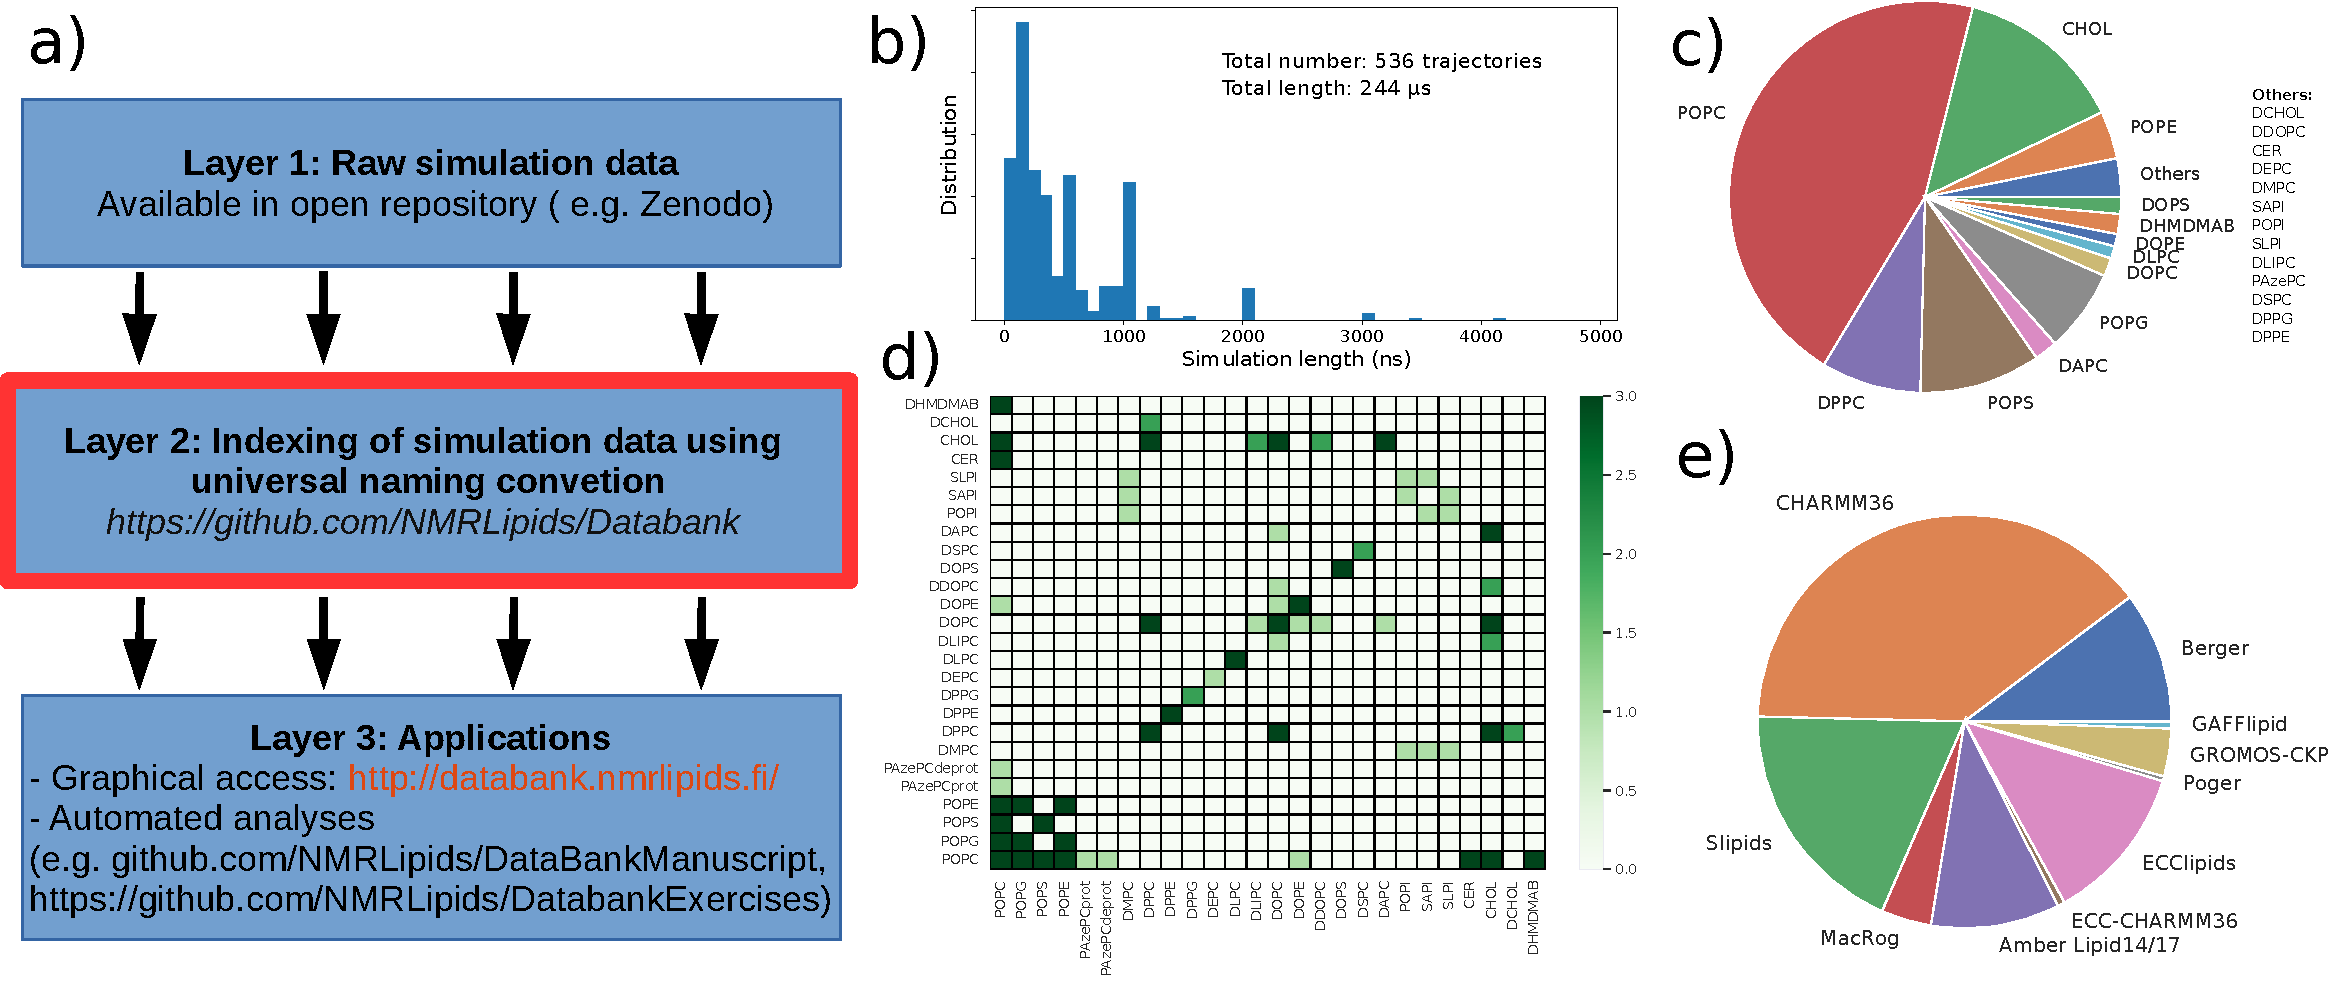
\includegraphics[width = 180mm]{Figures/overlay.pdf}
    \caption{a) Structure of an overlay databank. 
    %Raw data is available from a publicly accessible repository (layer 1).
    %The core of the databank contains information on the location of the raw data and indexing of molecular %compositions and simulation details described with universal naming conventions (layer 2).
    %The content of databank can be viewed and analysed using external programs that automatically read the information and data from layers 1 and 2 (layer 3). Examples of such applications are the GitHub repository generating the results presented in this work and the graphical access to the databank.
    More detailed structure of the layer 2 in the NMRlipids databank is illustrated in Fig.~\ref{DatabankStructure} in the SI.
    b) Distribution of the lengths of the trajectories, total number of trajectories and total lenght of the simulations in the NMRlipids databank.
    c) Distribution of lipids present in the trajectories in the NMRlipids databank. Lipids occuring in five or less simulations ('others') are listed in the right. 
    d) Currently available binary mixtures in the NMRlipids databank. 
    e) Distribution of force fields in the simulations in the NMRlipids databank.
    The figures and numbers are created on 9th of May 2022.}
    \label{fig:overlay}
\end{figure}

Currently the databank is composed of approximately 500 trajectories with the total length of approximately 231 microseconds of which most are contributed for the previous publications from the NMRlipids open collaboration~\cite{botan15,catte16,antila19,bacle21}. The distribution of lipids, force fields, length of the trjajectories and available binary mixtures are shown in Fig.~\ref{fig:overlay}. 

\subsection{Quality evaluation of force fields}
Quality of membrane simulations with different force fields have been evaluated against experimental data during parameterization and in separate comparison studies~\cite{botan15,ollila16,catte16,pluhackova16,perez17,leonard19}, but universal quality measure for membrane simulations is not defined and controversial results are often reported from simulations~\cite{antila22b}. The unclarities in simulation quality complicate the selection of proper simulation models for specific applications and estimation of reliability of reported simulation results, thereby being a major obstacle in many applications of membrane MD simulations.

To enable rapid evaluation and comparison of membrane MD simulation qualities, we define the quality measure for membrane MD simulations using the C-H bond order parameters from NMR experiments and form factors from x-ray scattering, which are robust experimental measurables that can be directly connected to the simulation data~\cite{ollila16}. C-H bond order parameters are related to the conformational ensemble of individual lipid molecules, while the form factor to arises from electron density thereby connecting to the overall structure of lipid bilayers. This is demonstrated in Fig.~\ref{fig:quality} a) showing correlations between membrane lateral density (area per lipid), thickness, minima of form factor and acyl chain order analyzed from all apporimately 500 trajectories in the NMRlipids databank. Membrane area per lipid has negative correlations with membrane order and thickness with Pearson coefficient of -0.78 and -0.49, respectively, because decreased area leads to more ordered, tightly packed and stretched acyl chains leading to thicker membranes. On the other hand, locations of form factor minima have positive correlation with the membrane area and negative correlation with the thickness. In conclusion, both x-ray scattering form factors and acyl chain order parameters from NMR are on average good proxies for membrane packing and thickness, while NMR order parameters give segmental resolution information on the quality of conformational ensembles of lipids.

\begin{figure}[tbp]
    \centering
    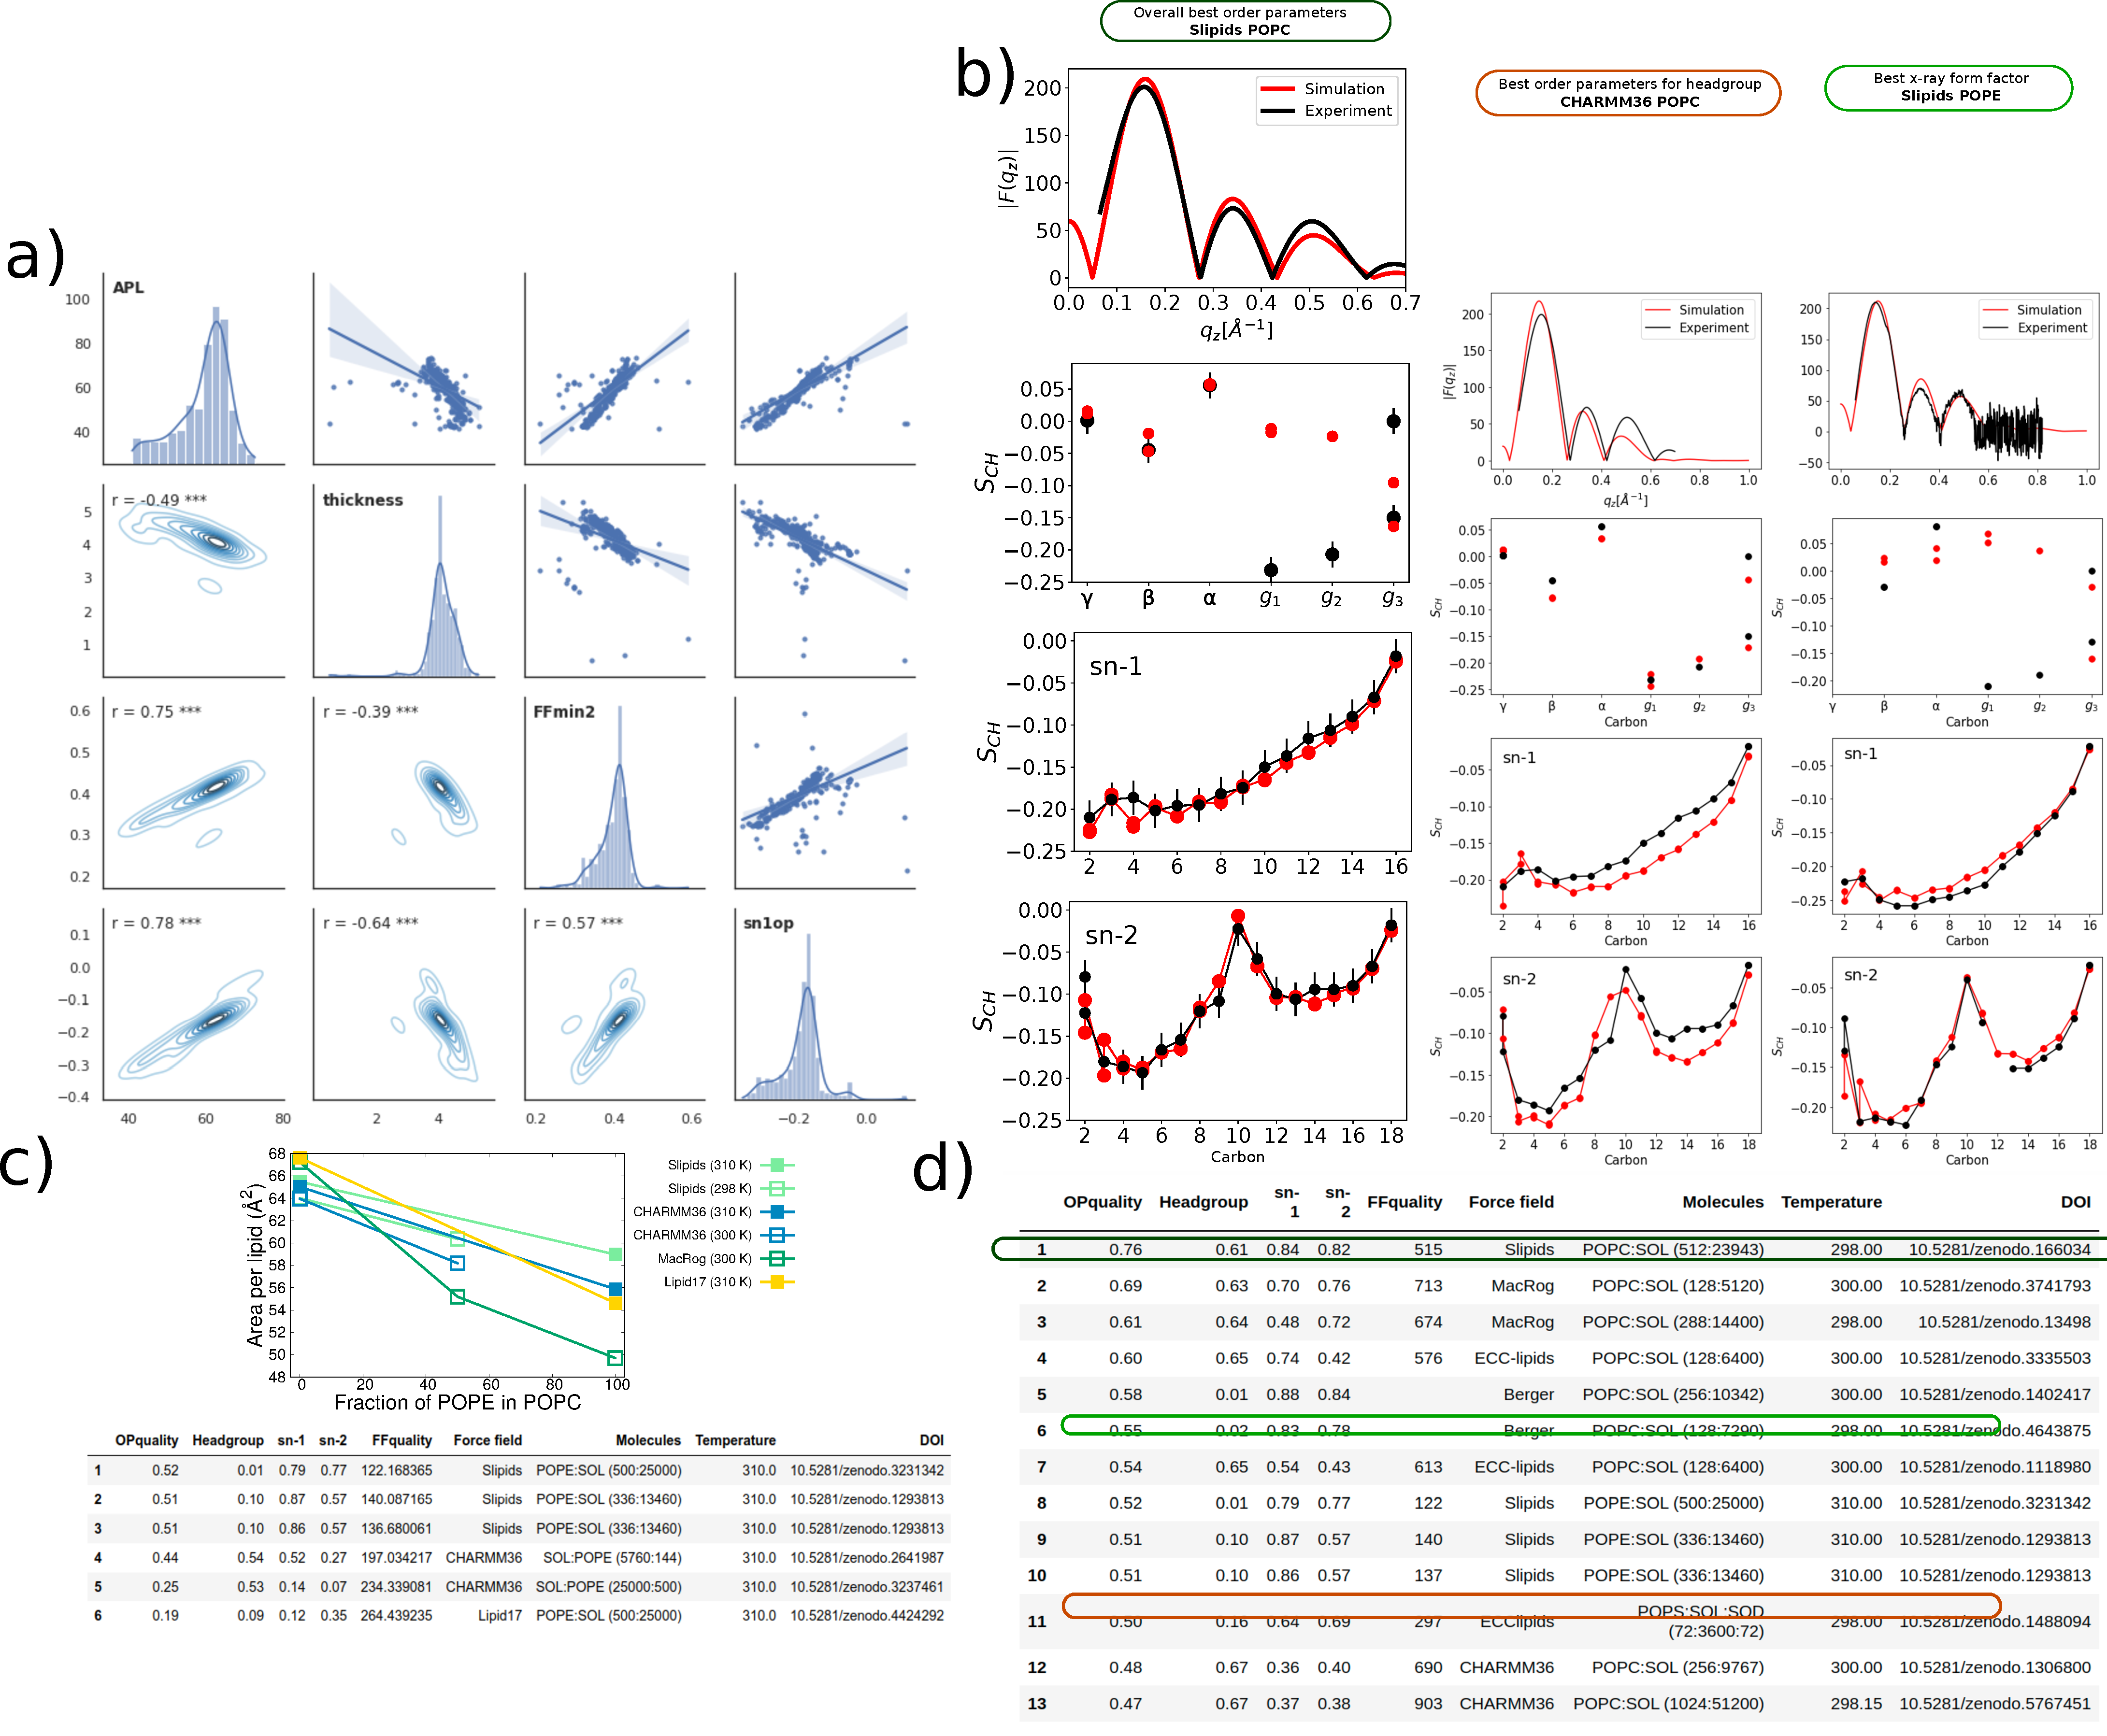
\includegraphics[width=180mm]{Figures/quality.pdf}
    \caption{a) Correlations between membrane area per lipid, thickness, second minima of form factor and average order parameter of the {\it sn}-1 acyl chain extracted from the NMRlipids databank. All Pearson correlation coefficients shown in bottom left corner have p-value below 0.001.
    b) Evaluation against experimental data exemplified for the simulation giving the best qualities in overall, for headgroup and x-ray scattering form factor.
    c) Change in area per lipid upon addition of POPE to POPC in different simulation extracted from the NMRlipids databank and quality evaluation table of POPE simulations.
    d) Quality evaluation table showing the best 13 simulations according to the overall order parameter quality.}
    \label{fig:quality}
\end{figure}

NMRlipids databank contains also experimental order parameter and x-ray form factor data that is connected to corresponding  simulations in order to define the simulation qualities and rank them to select the suitable simulation models for particular applications. The ranking of all simulations based on estimated average probability of order parameters to locate within experimental errors are shown in Fig.~\ref{fig:quality} b) and the comparison for the best models for overall quality, headgroup and glycerol backbone, and form factor are exemplified in Fig.~\ref{fig:quality} d). Full details of the NMRlipids quality measure for lipid bilayer simulations are given in the methods section and supplementary information.
The top ranking simulations in Figs.~\ref{fig:quality} b) and d) demonstrate also the current complexity in lipid bilayer simulation quality. Simulation of POPC lipid bilayer with Slipids force field ranks first in overall score, glycerol backbone is not correcetly captured in this model. On the othere, simulation with the best quality for headroup and glycerol backbone, CHARMM36 POPC, predicts too ordered acyl chain, thereby not being within the top 10 simulations in the overall ranking. The best ranking for x-ray form factor is given by the Slipids POPE simulation, however, because the quantitative value for form factor quality depends on the quality of experimental data, form factor qualities can be compared only between simulations evaluated against the same experimental dataset.

The power of NMRlipids quality metrics in selecting the best model for particular application is demontrated in Fig.~\ref{fig:quality} c) where the area per lipids of POPC:POPE mixtures from different force fields are shown and quality of POPE simulation in different force fields are evaluated. Among the simulations available in the NMRlipids databank, the Slipids force field gives the best quality in terms of acyl chain order parameters and form factor, and predicts the largest area per molecule for POPE and smallest difference with POPC. In conclusion, simulations with Slipids is the most reliable force field for membrane packing in POPC:POPE mixtures althought its glycerol backbone is not accurately modelled. Similar comparisons utilizing the preliminary data from the NMRlipids databank have concluded that Slipids is relatively good model also for mixtures of charged POPC:POPS membranes, although models with better counterion binding have higher quality, but CHARMM36 is the best to study differences in headgroup conformational ensembles between different lipid types. Understanding such complex picture of lipid bilayer MD simulation quality would not be possible without automatic quality evaluation of large sets of simulations enabled by the NMRlipids databank.

\subsection{NMRlipids databank reveals correlations between membrane properties}
The power of NMRlipids databank to find correlation between membrane properties is exemplified in Fig.~\ref{??} showing how water diffusion through and along the membrane correlate with different properties of systems. While NMRlipids databank enables similar analyses for any membrane properties, these are selected due to their relevance in the development of MRI imaging methods~\cite{??}.  


%\subsection{Spin relaxation rates of confined water close to membranes}

%Usefulness of the databank beyond MD simulation experts is demonstrated by analysing water spin relaxation times close to bilayers which are used in MRI imaging.

%Example text under a subsection. Bulleted lists may be used where appropriate, e.g.

%\begin{itemize}
%\item First item
%\item Second item
%\end{itemize}

%\subsubsection*{Third-level section}
 
%Topical subheadings are allowed.

\section{Discussion}

%The Discussion should be succinct and must not contain subheadings.

Quality measure and automatic quality evaluation of lipid bilayer MD simulations introduced in the NMRlipids databank enables rapid ranking of available simulation models agains experimental NMR and x-ray scattering data. This provides a tool for researches to rapidly evaluate the credibility of MD simulations of their own and reported by other groups. Because such tool and quality measure has not been available, this will elaborate the quality of published MD simulations of lipid bilyers and reduce potentially misleading results~\cite{antila22b}. The power of NMRlipids databank to select the best models for particular applications has been demontrated for PC/PE lipid mixtures (Fig.~\ref{fig:quality}), PC/PS lipid mixtures~\cite{antila22b}, and lipid headgroups~\cite{bacle21}.

The increasing amount of MD simulation data with programmatic access in the NMRlipids databank opens up possibilities for wide range of applications utilizing the large set of accessible data. Extend of the data in the NMRlipids databank in terms of quantity (e.g., simulation length and number of conformations), content (e.g, lipid compositions and ion concentrations) and quality enables analyses that are not possible to conduct from MD simulation data produced by a single research group. Applications of the NMRlipids databank to understand how diffusion of water through and along cellular membrane depends on its physical properties are demonstrated in Fig.~\ref{??}. Permeation of water through membranes resembles the permeation of also other hydrophilic molecules, such as drugs, and detailed understanding of water dynamics through and along membranes is potentially useful for the development of MRI imaging methods~\cite{topgaard20}. 
These examples demonstrate the practical applications of NMRlipids databank on problems in the biological and biomedical sciences.

Building accessible databanks of molecular dynamics simulation data has been challenging due to the required long term support for hardware and software maintenance. In the overlay model used in the NMRlipids databank, the demand of hardware can be distributed and open collaboration model reduces the risk for ending software maintenance. Furthermore, the open collaboration model used in the NMRlipids project credits contributors by offering authorship in published articles, thereby creating an incentive for contributions. This model could be extended also to other fields where similar barriers to establish publicly accessible databanks exist. Emerging applications of machine learning are increasing the impact of such databanks. For example, the existing Protein Databank (PDB)~\cite{??} containing experimentally determined protein structures with programmatic access has enabled the development of machine learning based tools building on the data collected in the databank over the years~\cite{??}. NMRlipids and other databanks with open programmatic access have potential to lead similar unforeseen applications in the future.


\section{Methods}

%Topical subheadings are allowed. Authors must ensure that their Methods section includes adequate experimental and characterization data necessary for others in the field to reproduce their work.

\subsection{Structure of the databank}

\begin{figure}
  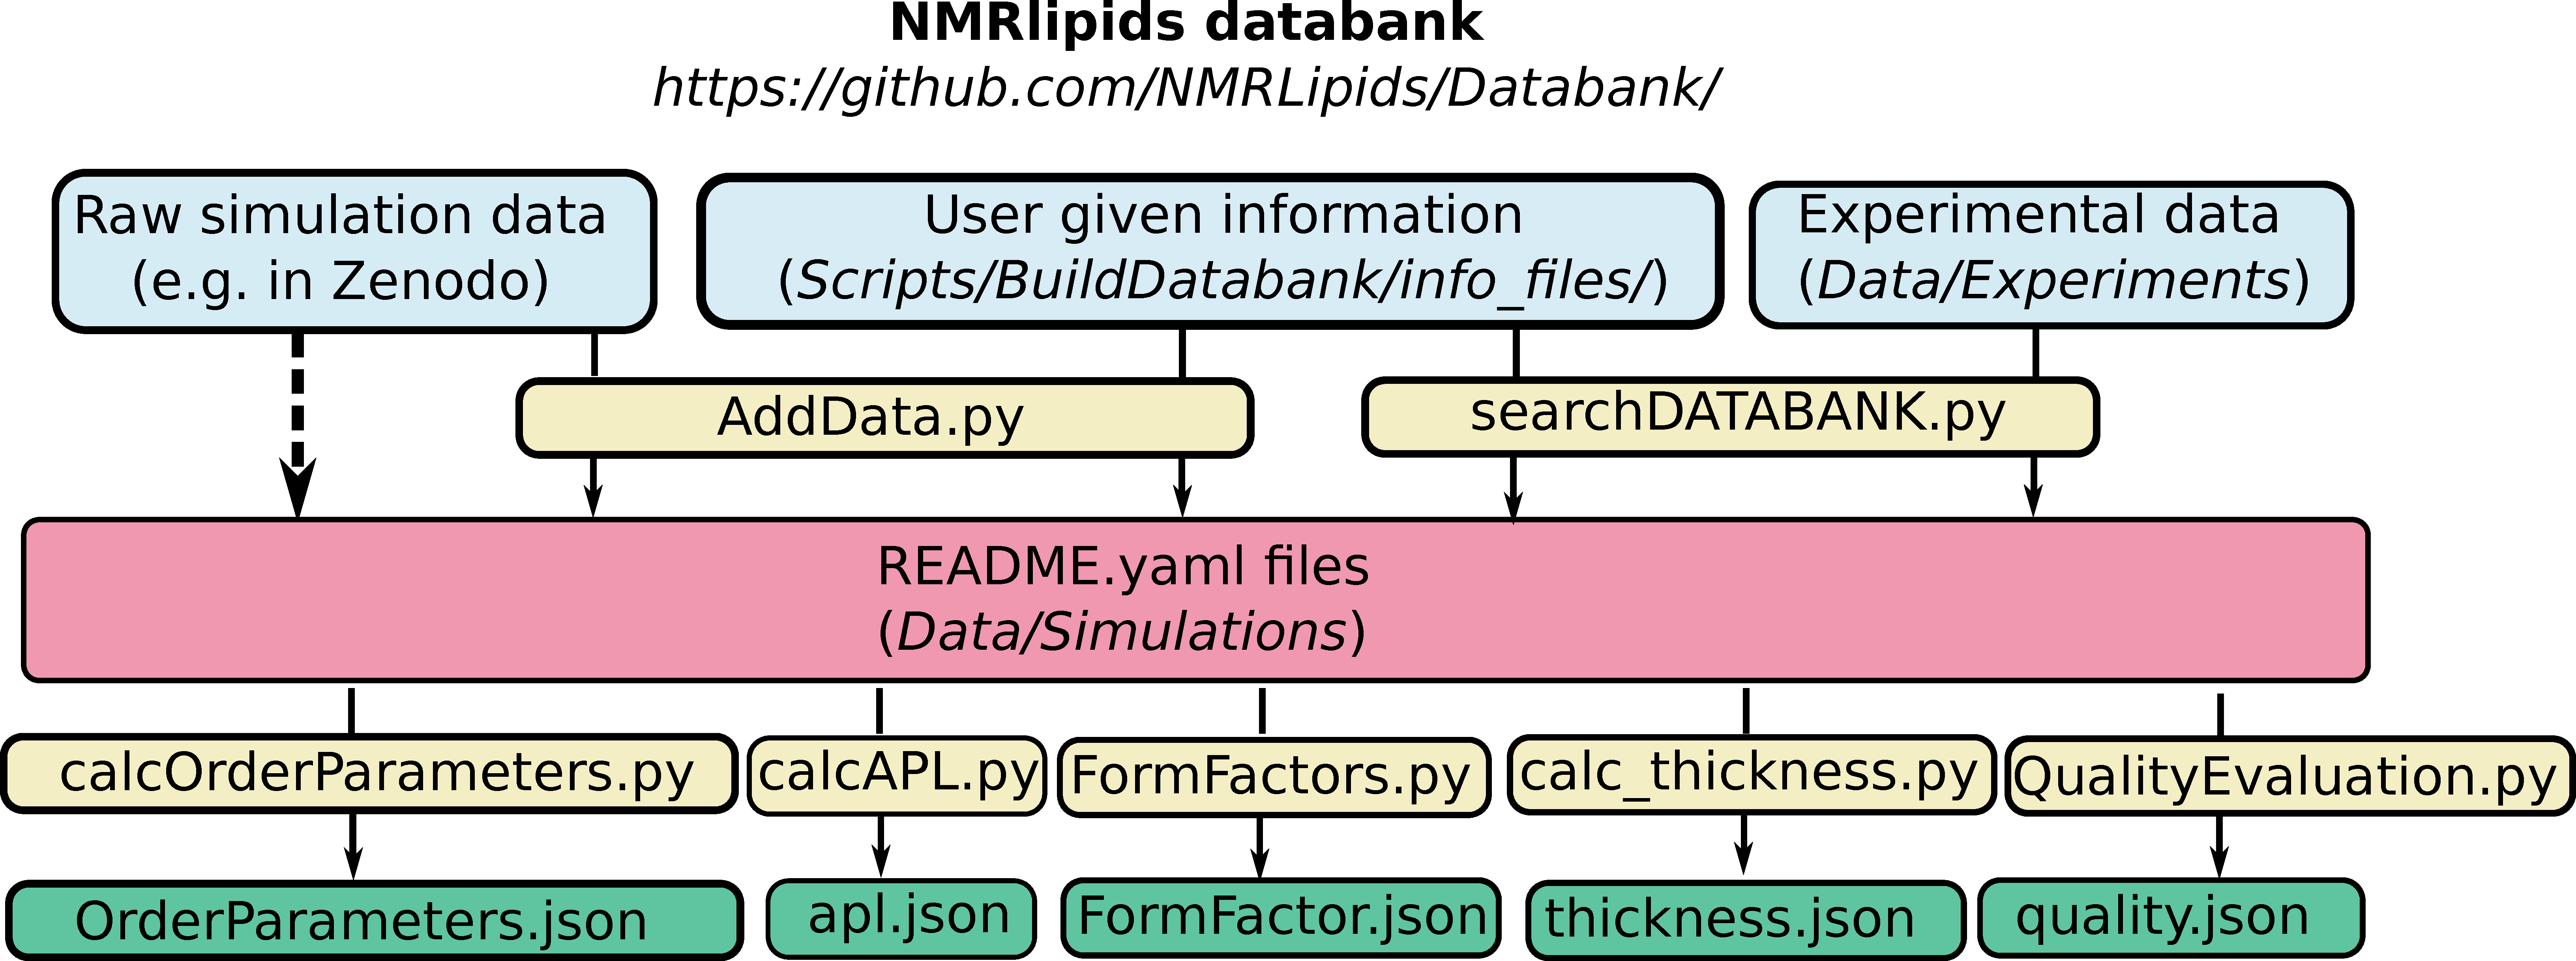
\includegraphics[width=\textwidth]{Figures/DataBankChart.pdf}
  \caption{Structure of the NMRlipids databank. Manually added input data (blue boxes) includes basic information on the simulation, permanent links to the raw data, and experimental data if available. The databank entries (red box) and analysis results (green boxes), locating at \url{https://github.com/NMRLipids/Databank/tree/main/Data/Simulations} are automatically generated by the computer programs included in the NMRlipids databank (yellow boxes). Because raw data are not permanently stored but can be accessed based on the information in the databank, this connection is marked with the dashed line. }\label{DatabankStructure}
\end{figure}

Structure of the NMRlipids databank is illustrated in Fig.~\ref{DatabankStructure}. The required input information to create an entry into the NMRlipids databank are listed in table~\ref{tab:READMEkeys}. While the raw simulation data is not directly stored in the NMRlipids databank, permanent links from where the raw data can be accessed have to be given and are then stored in the README.yaml files at \url{https://github.com/NMRLipids/Databank/tree/main/Data/Simulations}. These files contain all the essential information listed in table~\ref{tab:READMEkeys} on each simulation entry that are needed for further applications. The raw MD simulation data can locate in any stable publicly available repository, although all the current data locates in Zenodo \url{www.zenodo.org}. 

%A README.yaml file is made using AddData.py script for each simulation stored in the databank based on the information given by the author of the simulation data. In addition to this information, automatically extracted information about the simulation are stored in the README.yaml files (see table~\ref{tab:READMEkeys}). A README.yaml file for each simulation is stored to a folder named according to the hashes of original trajectory and topology file locating in \url{https://github.com/NMRLipids/Databank/tree/main/Data/Simulations}. These README.yaml files give access to all the essential information on the simulations in the databank either directly, or pointing to a original file from where the information can be extracted.

\begin{table}[]
    \centering
    \begin{tabular}{  p{3.5cm}  p{9.5cm}  p{4.0cm} }
    \toprule
    key & description & type  \\
    \midrule
        %\hline
    DOI & DOI from where the raw data is found & user given (compulsory) \\
    SOFTWARE & Software used to run the simulation (e.g. Gromacs, Amber, NAMD, etc.) & \\
    TRJ & Name of the trajectory file found from DOI & \\
    TPR & Name of the topology file found from DOI (trp file in the case of Gromacs) & \\
    PREEQTIME & Pre-equilibrate time simulated before the uploaded trajectory in nanoseconds. \tablefootnote{For example, if you upload 100-200 ns part of total 200 ns simulation, this should value should be 100.} & \\
    TIMELEFTOUT & Equilibration period in the uploaded trajectory that should be discarded in analyses. \tablefootnote{For example, if you upload 0-200 ns part of total 200 ns simulation where the first 100 ns should be considered as an equilibration, this value should be 100.} \\
    COMPOSITION & Molecules names used in the simulation and corresponding mapping files (see ??) & \\
    DIR\_WRK & Temporary working directory in your local computer. \\
    UNITEDATOM\_DICT & Information for constucting hydrogens for united atom simulations, empty for all atom simulations & \\
    TYPEOFSYSTEM & Lipid bilayer or something else & \\
    \hline
    PUBLICATION & Give reference to a publication(s) related to the data. & User given (optional)\\
    AUTHORS\_CONTACT & Name and email of the main author(s) of the data. & \\
    SYSTEM & System description on free text format & \\
    SOFTWARE\_VERSION & Version of the used software & \\
    FF & Name of the used force field & \\
    FF\_SOURCE & Source of the force field parameters, e.g, CHARMM-GUI, webpage, citation to a publication, etc. & \\
    FF\_DATE &  Date when force field parameters were accessed on the gives source (day/month/year). & \\
    FF{molename} & Molecule specific force field information, e.g., water model with FFSOL and sodium parameters with FFSOD. & \\
    CPT & Name of the Gromacs checkpoint file. & \\
    LOG & Name of the Gromacs log file. & \\
    TOP & Name of the Gromacs top file. & \\
    GRO & Name of the Gromacs gro file. & \\
    \hline
    TRAJECTORY\_SIZE & Size of the trajectory file in bytes & automatically extracted data. \\
    TRJLENGTH & Lenght of the trajectory (ps). & \\
    TEMPERATURE & Temperature of the simulation. & \\
    NUMBER\_OF\_ATOMS & Number of atoms in the simulation. & \\
    DATEOFRUNNIG & Date when added into the databank & \\
    EXPERIMENT & Potentially connected experimental data & \\
    COMPOSITION & Numbers of lipid molecules (NPOPC, NPOPG, etc.) per membrane leaflet are calculated by determining on which side of the center of mass of the membrane the center of mass of the head group of each lipid molecule is located.
    Numbers of other molecules such as solvent and ions (NSOL, NPOT, NSOD, etc.) are read from the topology file. & \\
    \end{tabular}
    \caption{Keys stored in the README.yaml files of simulations.}
    \label{tab:READMEkeys}
\end{table}

In order to evaluate the quality of simulations, sets of C-H bond order parameters from NMR and from factors from x-ray scattering are included in the NMRlipids databank (\url{https://github.com/NMRLipids/Databank/tree/main/Data/experiments}). The required information for an experimental dataset are listed in table~\ref{tab:READMEkeysEXP}.
A simulation is connected to a experimental data set
%C-H bond order parameter and x-ray scattering form factor data using the searchDATABANK.py script. Available experimental data is collected to  where each dataset is saved into a folder with the name based on DOI of the related publication and experimental conditions are described in README.yaml files with the keys listed in table~\ref{tab:READMEkeysEXP}. 
if molar concentrations of all molecules are within $\pm$5 percentage units, charged lipids have the same counterions, and temperature is within $\pm$2 degrees. In such cases, a simulation and experimental data are paired by adding the path to the experimental data into the simulation README.yaml file. 
%If lipid to water ratio is above ??, the systems are considered fully hydrated. Otherwise also hydration level is considered.

\begin{table}[]
    \centering
    \begin{tabular}{  p{5.0cm}  p{10.0cm}}
    \toprule
    key & description \\
    \midrule
    DOI & DOI of the publication related to the experimental data. \\
    TEMPERATURE & Temperature of the experiment. \\
    MOLAR\_FRACTIONS & Dictionary of molar fractions of bilayer components \\
    ION\_CONCENTRATIONS & Dictionary of ion concentrations of the system (defined as ??) \\
    TOTAL\_LIPID\_CONCENTRATION & Total concentration of lipid components. If exact concentration is not known, but experiments are performed in excess water, 'full hydration' can be given. \\
    COUNTER\_IONS & Type of counter ions if present.
\end{tabular}
    \caption{Keys stored in the README.yaml files of experiments.}
    \label{tab:READMEkeysEXP}
\end{table}

Because README.yaml contains all the essential information on each simulation, arbitrary analyses can be automatically performed over all the simualtions in the NMRlipids databank. In addition to the order parameters for each C-bonds and x-ray scattering form factors used in the quality evaluation, the NMRlipids databank contains the area per lipid and thickness calculated from all simulations in the databank. These results are stored in the same folders as the README.yaml files in \url{https://github.com/NMRLipids/Databank/tree/main/Data/Simulations}.

\subsection{Molecule and atom naming convention}

Because universal convention for lipid molecules and atoms therein has not been defined, the naming conventions vary between authors and force fields. To enable automatic analyses over large sets of simulation in the NMRlipids databank, we have defined unique naming conventions for lipid molecules and atoms. The abbreviations of molecule names used in the NMRlipids databank are listed in table~\ref{tab:abbreviations}. The unique atom names for each molecule and corresponding names in each simulation are defined using mapping files introduced in the NMRlipids project (\url{https://nmrlipids.blogspot.com/2022/04/new-yaml-format-of-mapping-files.html}). 

Molecule and atom names in each simulation are connected to the unique naming convention with the COMPOSITION dictionary in the README.yaml file. Upon addition of a new entry in the databank, the molecule names in the simulation corresponding the unique names and mapping files (available at \url{https://github.com/NMRLipids/Databank/tree/main/Scripts/BuildDatabank/mapping_files}) are defined in the dictionary. The numbers of molecules in the system are then automatically calculated by the NMRlipids databank codes (AddData.py in Fig.~\ref{DatabankStructure}) and stored in the README.yaml together with other content of the COMPOSITION dictionary. This information can be then used to find each molecule and atom from each simulation in the analysis codes.  

\begin{table}[h]
    \centering
    \begin{tabular}{c|c}
        Abbreviation & Molecule name \\
        \hline
        POPC &  1-palmitoyl-2-oleoyl-sn-glycero-3-phosphocholine\\
        POPG &  1-palmitoyl-2-oleoyl-sn-glycero-3-phosphoglycerol \\
        POPS & 1-palmitoyl-2-oleoyl-sn-glycero-3-phospho-L-serine \\
        POPE & 1-palmitoyl-2-oleoyl-sn-glycero-3-phosphoethanolamine \\
        CHOL & cholesterol \\
        DHMDMAB & dihexadecyldimethylammonium \\
        \hline
        POT & potassium ion \\
        SOD & sodium ion \\
        CLA & chloride ion \\
        CAL & calcium ion \\
        SOL & water \\
    \end{tabular}
    \caption{Abbreviations used in the databank}
    \label{tab:abbreviations}
\end{table}


\subsection{Quality evaluation}

Quality of conformational ensembles of lipid molecules in simulations are evaluated by estimating the average probability of C-H bond order parameters to agree with the values from NMR experiments. 
%As a first step, the quality of each order parameter is evaluated using the negative logarithm of probability to find the simulated order parameter within the experimental error bars
%\begin{equation}
%    S_q = -\log_{10}(P),    
%\end{equation}
Because each C-H bond order parameter is calculated as an average over individual lipids in a simulation and conformational ensembles of lipids are assumed to be independent, the random variable
\begin{equation}
    \frac{\bar{X}-\mu}{S/\sqrt{n}},
\end{equation}
where $\bar{X}$ is the sample mean, $S$ is the sample variance and $n$ is the sample size (number of lipids), has a Student's t-distribution with $n-1$ degrees of freedom and the mean of $\mu$.


where the probability is calculated from the normal distribution
\begin{equation}\label{gaussian}
    P = \int_{S_{\rm exp}-\Delta S_{\rm exp}}^{S_{\rm exp}+
    \Delta S_{\rm exp}}  \frac{1}{\sigma \sqrt{2\pi}} e^{-\frac{1}{2}(\frac{x-\mu}{\sigma})^2} {\rm d}x.
\end{equation}
$S_{\rm exp}$ and $\Delta S_{\rm exp}$ are experimental order parameter and its error, and $\mu$ and $\sigma$ are the mean order parameter and its standard deviation from simulations. The quality measure $S_q$ approaches to zero when probability for agreement between simulation and experimental results approach one, and increases when simulated and experimental values diverge. The accuracy of $\pm$0.02 is currently assumed for all experimental order parameters~\cite{ollila16}. Because phospholipids sample their conformational ensemble within nanosecond timescale~\cite{ferreira15}, all simulations in the databank would be sufficiently long to sample the realistic conformational phase of individual lipids. However, some force fields exhibit too slow dynamics which leads to large error bars in order parameter values~\cite{antila21a}. Because large error bars widen the gaussian distribution in Eq.~\ref{gaussian} thereby artificially increasing the probability to find the simulated value within experimental error bars, the order parameters with error bars larger than the experimental error 0.02 are not included in the quality evaluation.

The quality of separate fragments in each lipid type within a simulation are then evaluated by averaging individual order parameter qualities over C-H bond belonging to that fragment and dividing this with the percentage of order parameters for which the quality is available within the fragment, $p$
\begin{equation}
    S_q^{\rm frag}[{\rm lipid}] = \frac{\langle S_q[{\rm lipid}]\rangle_{\rm frag}}{p_{\rm frag}[{\rm lipid}]},
\end{equation}
 where frag can be {\it sn}-1, {\it sn}-2, headgroup or total (all order parameters within a molecule). The overall quality of different fragments in a simulation are then defined as a molar fraction weighted average over different lipid components
\begin{equation}
    S_q^{\rm frag} = \sum_{\rm lipid} \chi_{\rm lipid} \langle S_q^{\rm frag}[{\rm lipid}]\rangle_{\rm lipid} ,
\end{equation}
where $\chi_{\rm lipid}$ is the molar fraction of a lipid in the bilayer.

Qualities of form factors were evaluated with the same approach that was used in SIMtoEXP program~\cite{kucerka10}. Because experiments give form factors only in relative scale those were scaled to the simulation data with absolute scale using equation
\begin{equation}
    k_e = \frac{\sum_{i=1}^{N_q} \frac{|F_s(q_i)||F_e(q_i)|}{(\Delta F_e(q_i))^2}}{\sum_{i=1}^{N_q} \frac{|F_e(q_i)|^2}{(\Delta F_e(q_i))^2}}.
\end{equation}
The quality of each form factor was then calculated from the equation
\begin{equation}
    \chi^2 = \frac{\sqrt{\sum_{i=1}^{N_q}(|F_s(q_i)|-k_e|F_e(q_i)|)^2/(\Delta F_e(q_i))^2}}{\sqrt{N_q-1}},
\end{equation}
where $F_s$ and $F_e$ are form factors from a simulation and experiment, respectively, and summation goes over the experimentally available $N_q$ points. 



\subsection{Analysing simulations in the NMRlipids databank}

The README.yaml files contain all the essential information to perform arbitrary analyses of simulations in the NMRlipids databank, i.e., the permanent location of the original data and naming convention for all atoms and molecules in each system. In practise, the analyse codes contains a loop over all README.yaml files (i.e., simulations in the NMRlipids databank) which first downloads the raw simulation to a local computer and then uses the information about the atom and molecule naming conventions in README.yaml and mapping files to perform the desired analyses. For example, the code that calculates all C-H bond order parameters of all systems is available at \url{https://github.com/NMRLipids/Databank/blob/main/Scripts/AnalyzeDatabank/calcOrderParameters.py} and minimal example of a analysis code is available at \url{https://github.com/NMRLipids/Databank/blob/main/Scripts/AnalyzeDatabank/template.ipynb}.

While the order parameters, form factors, area per lipid and thickness are stored within the NMRlipids databank (\url{https://github.com/NMRLipids/Databank/tree/main/Data/Simulations}), further analyses can be conventiently stored in separate repositories with the same folder structure based on hash identities of trajectory and topology files. For example, results from further analyses performed here are stored in folders at \url{https://github.com/NMRLipids/DataBankManuscript/tree/main/Data}. Such organization of the data enables further upcycling of the analyzed data as similarly to the original NMRlipids databank repository.

%\subsection{Indexing the simulation data}

%\subsubsection*{AddData.py}
%AddData.py is a script that builds a database that contains a dictionary file and analysis data of each simulation. The dictionary file contains information about the simulation. The script also calculates order parameters of all CH bonds of the lipids in the simulation. To add a simulation it must be first uploaded to Zenodo (www.zenodo.org). The trajectory and topology files of the simulation are downloaded to the working directory from Zenodo but these are not saved into the database. To add a simulation to the database the user has to give some essential information about the simulation. This is done by writing a info file (*INFO.yaml) which is passed to AddData.py. 
%\newline \\
%AddData.py requires GROMACS and MDAnalysis library to be installed.
%\newline \\
%Run AddData.py as follows:
%\newline \\
%python3 AddData.py -f exampleINFO.yaml
%\newline \\
%There is also a script runAddData.sh that can be used to loop over several info files to add many simulations at one go.

%\subsubsection*{Simulation dictionary}
%A simulation dictionary contains information about the simulation. Some of the information is provided by the user. The numbers of lipid molecules, solvent and ions are automatically read from the files and so are the simulation temperature and trajectory length. All this information is saved to a file named README.yaml.


%\subsubsection{User input}
%Dictionary variables defined by the user are listed here. 
%The necessary parameters required for the analyses are described first and are marked as ''compulsory''. Then the parameters used to describe the data for further usage and analyses are described.
%While only compulsory parameters are required for the databank entry, strong recommendation is that all the possible parameters would be given to maximize the possibilities to upcycle the contributed data. 

%\subsubsection*{DOI (compulsory)}
%Give DOI identity from where the simulation files are located. Current databank works only for the data in Zenodo, but other potential sources are may be implemented in the future. Note that the DOI must point to a specific version of dataset in Zenodo, i.e., DOI pointing to all versions of certain dataset does not work.

%\subsubsection*{SOFTWARE (compulsory)}
%Give the name of software used to run the simulation. The options are GROMACS, AMBER, NAMD, CHARMM and OPENMM. So far, only simulations run with GROMACS are accepted by the script.

%\subsubsection*{TRJ (compulsory)}
%Give the name of the trajectory file that is found from the DOI given above.

%\subsubsection*{TPR (compulsory)}
%Give the name of the file with topology information (tpr file in the case of Gromacs) that is found from the DOI given above.

%\subsubsection*{PREEQTIME (compulsory)}
%Give the time simulated before the uploaded trajectory in nanoseconds. For example, if you upload 100-200~ns part of total 200~ns simulation, this should value should be 100.

%\subsubsection*{TIMELEFTOUT (compulsory)}
%Give the time that should be considered as an equilibration period in the uploaded trajectory. Frames before the give time will be discarded in the analysis. For example, if you upload 0-200~ns part of total 200~ns simulation where the first 100~ns should be considered as an equilibration, this value should be 100.


%\subsubsection*{Molecule names (compulsory)}
%In the databank, each molecule has a unique abbreviation (see table~\ref{tab:abbreviations}). 
%You need to give the residue names of these molecules corresponding your simulation.
%The user must also provide the names of the molecules, ions and solvent that are used in the simulation to match the names used by the databank. The names provided by the user must be the same as in the tpr file. 
%If atoms in a lipid belong to different residues (typical situation in Amber force fields), give the name of the head group residue here, and add the residue name of each atom to the third column in the mapping file (see below). If your simulation contains molecules that are not yet in the databank, you need to define the abbreviation and add molecules to the lipids\_dict, molecules\_dict, molecule\_numbers\_dict and molecule\_ff\_dict in the AddData.py script, as well as to table~\ref{tab:abbreviations}. 


%\subsubsection*{MAPPING\_DICT (compulsory)}
%For the analysis, we need to know the names of atoms in your system.
%These are defined using the mapping file convention introduced in \url{http://nmrlipids.blogspot.com/2015/03/mapping-scheme-for-lipid-atom-names-for.html}, where first column gives the universal atom name, second gives the atom name in force field, and third gives the residue name if not the same for all atoms.
%The name of the mapping file for each molecule needs to be given in dictionary format. The dictionary the key is the molecule name (abbreviation listed in table \ref{tab:abbreviations}) and the value is the name of the mapping file. The already existing mapping files can be found from the directory named "mapping\_files". If a mapping file for your molecule(s) do not exist, you need to construct one and add to the "mapping\_files" directory.

%\newline \\
%The purpose of a mapping file is to circumvent the problem caused by different atom naming conventions used by different force fields. The first column of a mapping file contains general atom names. The second column contains the name of the atom as it is in the force field. If the lipid consists of several residues which is the case in some AMBER force fields, then a third column is needed which contains the name of the residue to which each atom belongs to.

%\subsubsection*{DIR\_WRK (compulsory)}
%Give the path of the working directory in your local computer. The trajectory and topology files will be downloaded to this trajectory, and temporary files created during processing will be stored here. 


%\subsubsection*{UNITEDATOM\_DICT (compulsory for united atom trajectories)}
%Order parameters from united atom simulations are calculated using buildH code (\url{https://github.com/patrickfuchs/buildH}). For united atom simulations, you need to tell how hydrogens are added based on definitions in the dic\_lipids.py dictionary. This is done by giving a dictionary where the key is the molecule name (abbreviation listed in table \ref{tab:abbreviations}) and the value is the correct dictionary key in dic\_lipids.py. If correct dictionary key is not yet found, you need to add to dic\_lipids.py. 
%In the case of an all atom simulation, UNITEDATOM is left empty.


%\subsubsection*{PUBLICATION}
%Give reference to a publication(s) related to the data.

%\subsubsection*{AUTHORS\_CONTACT}
%Give the name and email of the main author(s) of the data.

%\subsubsection*{SYSTEM}
%Give description of system in free format. For example ''POPC with cholesterol at 301K''.


%\subsubsection*{SOFTWARE\_VERSION}
%Give the version of the software used.

%\subsubsection*{FF}
%Give the name of the force field used used in the simulation.

%\subsubsection*{FF\_SOURCE}
%Describe the source of the force field parameters. For example, CHARMM-GUI, link to webpage where parameters were downloaded, or citation to a paper.

%\subsubsection*{FF\_DATE}
%Give the date when parameters were accessed or created. The format is day/month/year.

%%\subsubsection*{Individual force field names for molecules}
%In some cases special force fields are used for certain molecules. For example, non-standard parameters for ions or other molecules have been used. These can be specified giving forcefield names separately for individual molecules. These can be given as parameters named as
%FF+[abbreviation from table \ref{tab:abbreviations}], i.e., FFPOPC, FFPOT, FFSOL etc.

%\subsubsection*{CPT (Gromacs)}
%Give the name of the Gromacs checkpoint file that is found from the DOI given above.
%CPT stands for the name of the cpt file. 

%\subsubsection*{LOG (Gromacs)}
%Give the name of the Gromacs log file that is found from the DOI given above.

%\subsubsection*{TOP (Gromacs)}
%Give the name of the Gromacs top file that is found from the DOI given above.



%\subsubsection{Automatically analyzed parameters}
%The following parameters are read automatically from the trajectory and topology files.
%%%%%%%%%%%%%%%%%%%%%%%%%%%%automatically analyzed parameters%%%%%%%%%%%%%%%%%%%%%%%%%%%%%%


%\subsubsection*{Molecule numbers}
%Numbers of lipid molecules (NPOPC, NPOPG, etc.) per membrane leaflet are calculated by determining on which side of the center of mass of the membrane the center of mass of the head group of each lipid molecule is located.
%\newline \\
%\noindent Numbers of other molecules such as solvent and ions (NSOL, NPOT, NSOD, etc.) are read from the topology file.

%\subsubsection*{Temperature}
%Temperature of the simulation is read from the topology file.

%\subsubsection*{Trajectory length}
%The length of a trajectory is read from the trajectory file.

%\subsubsection*{Date of running}
%The date of running the script is saved to the README.yaml file.



\bibliography{refs.bib}

%\noindent LaTeX formats citations and references automatically using the bibliography records in your .bib file, which you can edit via the project menu. Use the cite command for an inline citation, e.g.  \cite{Hao:gidmaps:2014}.

%For data citations of datasets uploaded to e.g. \emph{figshare}, please use the \verb|howpublished| option in the bib entry to specify the platform and the link, as in the \verb|Hao:gidmaps:2014| example in the sample bibliography file.

\section*{Acknowledgements}

%Acknowledgements should be brief, and should not include thanks to anonymous referees and editors, or effusive comments. Grant or contribution numbers may be acknowledged.

\section*{Author contributions statement}

Must include all authors, identified by initials, for example:
A.A. conceived the experiment(s),  A.A. and B.A. conducted the experiment(s), C.A. and D.A. analysed the results.  All authors reviewed the manuscript. 

\section*{Additional information}

%To include, in this order: \textbf{Accession codes} (where applicable); \textbf{Competing interests} (mandatory statement). 

%The corresponding author is responsible for submitting a \href{http://www.nature.com/srep/policies/index.html#competing}{competing interests statement} on behalf of all authors of the paper. This statement must be included in the submitted article file.

%\begin{figure}[ht]
%\centering
%
\includegraphics[width=\linewidth]{stream}
%%\caption{Legend (350 words max). Example legend text.}
%\label{fig:stream}
%\end{figure}

%\begin{table}[ht]
%\centering
%\begin{tabular}{|l|l|l|}
%\hline
%Condition & n & p \\
%\hline
%A & 5 & 0.1 \\
%\hline
%B & 10 & 0.01 \\
%\hline
%\end{tabular}
%\caption{\label{tab:example}Legend (350 words max). Example legend text.}
%\end{table}

%Figures and tables can be referenced in LaTeX using the ref command, e.g. Figure \ref{fig:stream} and Table \ref{tab:example}.

\end{document}
